

\section{The \textsc{RippleEval} Benchmark}
\label{sec:dataset}


To comprehensively analyze how factual updates affect related knowledge after post-training, we construct \textbf{\textsc{RippleEval}}, a QA-based benchmark grounded in verified factual relations. 

Each QA sample in \textsc{RippleEval} corresponds to an underlying factual relation $(s,r,o)$, where $s$ and $o$ are entities and $r$ is a relation. We use these grounded relations to connect QA samples because QA expressions themselves are not stable units for defining factual dependency: the same fact can be asked in different ways, while unrelated facts may share similar question templates. Thus, the graph is used to define factual connections among QA samples, while model training and evaluation are still performed through natural-language QA.

\paragraph{Grounded Graph Construction.}
We construct an entity-level factual graph and use it to organize QA samples. In this graph, each node is an entity, and each directed edge represents a verified factual relation $(s,r,o)$ from subject entity $s$ to object entity $o$ under relation $r$. Each verified edge is then verbalized into a QA sample for training and evaluation.

\paragraph{Graph Construction under Constrainted Relations.}
In ripple-effect evaluation, an edited fact is expected to change or preserve the answers to a set of related factual queries. To determine whether such downstream behavior is correct, each query must have an unambiguous target answer. This becomes problematic for one-to-many relations: for a subject--relation pair with multiple valid objects, a model prediction may differ from the annotated object while still being factually correct. Such ambiguity would make it unclear whether an apparent mismatch reflects an incorrect ripple effect or an incomplete annotation.

To avoid this issue, \textsc{RippleEval} restricts evaluation to subject--relation pairs $(s,r)$ with a unique or primary expected object $o$. Relations such as \textit{CapitalOf} and \textit{DevelopedByPrimary} satisfy this requirement, whereas relations such as \textit{HasChild} are excluded because they may have multiple valid objects. 

This design differs from prior benchmarks such as MQUAKE \cite{zhong2023mquake} and RippleEdits \cite{cohen2023ripple}, which evaluate whether model edits lead to correct multi-hop or downstream consequences, but do not explicitly control the answer cardinality of each queried subject--relation pair. By enforcing this constraint, \textsc{RippleEval} can construct controlled factual neighborhoods whose ripple-effect targets are uniquely specified.


\paragraph{Expansion and Verification.}
We construct the factual grounding graph $\mathcal{G}_{fact}$ with an automated expansion-and-filtering pipeline. Starting from high-confidence seed triplets, such as \texttt{("Minecraft", "DevelopedByPrimary", "Mojang Studios")}, we iteratively expand from the entities reached so far using a predefined set of factual relations. During expansion, we discard any triplet whose object entity already appears earlier on the same path. This removes cyclic dependencies, where a later hop points back to an ancestor entity, and ensures that retained paths represent genuine downstream factual connections. We then verify the retained triplets and remove cases with unsupported, ambiguous, or non-primary objects.

\paragraph{Scaling Up Knowledge Graph.}
Instead of relying on small-scale local models, we utilize the high-throughput DeepSeek API (\texttt{deepseek-chat}) to simultaneously propose candidate triplets and generate high-quality natural language questions. Scaling this rigorous generation process consumed approximately 309.2 million tokens (182.6M prompt, 126.6M completion). Crucially, the generated questions are hardcoded directly into the graph's edge attributes. This mechanism strictly eliminates prompt variance during evaluation: models are tested using the exact same question string before and after the update, ensuring failures stem from structural corruption rather than wording ambiguity. Each candidate is then verified against Wikidata \cite{vrandecic2014wikidata} through an external validation module, and unverified triplets are discarded. The final graph $\mathcal{G}_{fact}$ comprises $100,015$ unique entity nodes and $432,562$ verified relation edges spanning 39 strict relation types.

\paragraph{Factual Connectivity as Popularity.}
After constructing the verified factual graph, we use entity connectivity to approximate the popularity of factual knowledge in the benchmark. For a factual relation $(s,r,o)$, we measure the connectivity of its object entity $o$ by its in-degree, i.e., how many verified subject-relation facts point to the same object. This score does not measure how often a QA wording appears; instead, it measures how widely the answer entity is shared across different factual relations.

This definition gives each QA sample a grounded popularity score through its underlying factual relation. A sample whose answer entity is connected to many other facts is treated as involving a more widely shared factual anchor, while a sample whose answer entity has few incoming facts is treated as involving a narrower factual context. In this way, the graph connectivity serves as a proxy for the uneven distribution of real-world knowledge, where some entities are linked to many facts and others are much more isolated.

\paragraph{External Validation of the Popularity Proxy.}
Because in-degree is defined entirely within $\mathcal{G}_{fact}$, it is not immediately clear whether it tracks any externally observable notion of popularity. To verify that it does, we compare in-degree against two independent corpus-level signals on the QID-resolved subset of the graph: (i) the per-entity surface-form frequency in $200{,}000$ English Wikipedia articles ($\approx 100$M tokens, matched with an Aho--Corasick automaton), and (ii) the $2024$ Wikipedia pageview total of the entity's article (user-agent only). After restricting to nodes for which all three signals are non-zero, $35{,}868$ entities remain ($59.9\%$ of QID-resolved nodes). On this set, the pairwise log-log Spearman rank correlations are $\rho(\text{in-degree}, \text{wiki frequency}) = +0.308$, $\rho(\text{in-degree}, \text{pageviews}) = +0.235$, and $\rho(\text{pageviews}, \text{wiki frequency}) = +0.351$ (all $p \approx 0$; Figure~\ref{fig:popularity_proxy}). The three signals are therefore consistently and positively related, yet none reaches $\rho = 0.4$, indicating that they capture related but non-redundant aspects of factual prominence rather than the same underlying quantity.

The agreement is strongest at the head of the distribution: among the top-$10$ entities ranked by wiki frequency, $8$ also fall in the top decile by in-degree, and $\mathrm{United\ States}$ (Q30) is the maximum on both axes. The disagreement is concentrated in two complementary regimes. First, entities that are densely interlinked in $\mathcal{G}_{fact}$ but rare in Wikipedia surface text (e.g., $\mathit{ESPN}$, $\mathit{Dell\ Technologies}$, $\mathit{Assembly\ language}$; each with in-degree $\ge 15$ and $\mathrm{wiki\ frequency} = 1$) are recognized as factual anchors by in-degree but not by raw corpus frequency. Second, entities with high public attention but sparse factual annotations in $\mathcal{G}_{fact}$ (e.g., recent public figures and events with large pageviews and small in-degree) are recognized by pageviews but not by in-degree. In both cases the disagreement is structural rather than noise: in-degree measures how many distinct verified factual relations resolve to an entity, which is the property our ripple-effect analyses depend on. We therefore retain in-degree as the popularity proxy in Sections~\ref{sec:setup}--\ref{sec:results}, and treat wiki frequency and pageviews as external corroboration rather than as substitutes.

\begin{figure}[t]
    \centering
    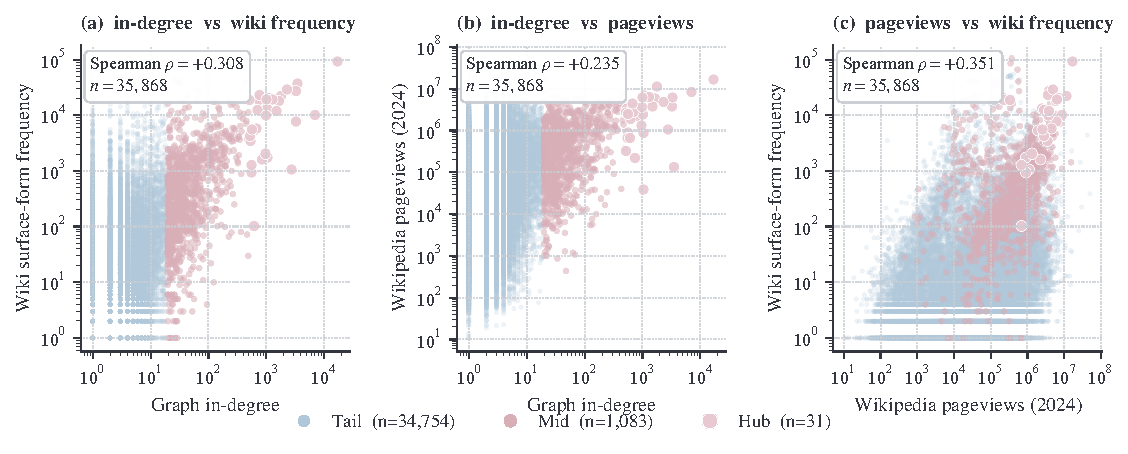
\includegraphics[width=\columnwidth]{figures/Fig1_PopularityProxy.pdf}
    \caption{\textbf{External validation of the popularity proxy.} Pairwise log-log scatter of graph in-degree, $2024$ Wikipedia pageviews, and entity surface-form frequency in $200$k English Wikipedia articles, on the $35{,}868$ QID-resolved nodes of $\mathcal{G}_{fact}$ for which all three signals are non-zero. Each panel reports the Spearman rank correlation. The three signals are consistently positively related (all $\rho > 0.2$) but none reaches $\rho = 0.4$, indicating non-redundant aspects of factual prominence. Hub, Mid, and Tail strata are defined by in-degree thresholds; hub points are plotted on top for visibility.}
    \label{fig:popularity_proxy}
\end{figure}

